\documentclass[upLatex]{jsreport}
\usepackage{siunitx} % SI unit
\usepackage[dvipdfmx]{graphicx} % Put on pictures
\usepackage{float} % put on images on my own way
\usepackage{remreset} % configure fig. number

\begin{document}

\tableofcontents

\newpage
\chapter{序論}
\section{研究背景}
コウモリは,超音波を放射し,周囲からのエコーを脳内で処理することで
空間情報を高度に取得している(エコーロケーション行動).
このコウモリが日常的に行っているエコーロケーション行動は,
音響計測を通じた行動実験や,
ボトムアップ的に行われている神経生理学的実験等により,
生物学的のみならず,
工学的にもユニークであり優れていることが解明されてきている[1,2].
しかし従来からのこれらの実験では,
コウモリが与えられた環境に対して,
どのような行動を示すかを計測することはできるが,
“なぜそのような行動を選択するのか”という,
コウモリの意思判断の基準やルールは推測するしかなかった.

一方で,近年発展が著しい機械学習分野の生物学分野への融合が図られ始め,
特に報酬と行動との関連を学習する強化学習・逆強化学習を
生物の行動研究に応用する例も出始めている[3,4].

\section{研究目的}
本研究では,コウモリの飛行とパルス放射方向を決定する環境因子の
同定を目的に,コウモリの飛行実験を模擬したシミュレーション実験を行った.
コウモリを模擬したエージェントは強化学習によって最適な飛行方策を学習する.
設定した報酬により,どのような行動を選択するのかを検討することで,
コウモリが重要視しているパラメータを推定し,
実際の飛行実験により得られた行動と比較した.


\newpage
\chapter{強化学習}
強化学習では,環境と,環境内で行動するエージェントをそれぞれ定義する.
エージェントはある時間$t$において,環境から状態$s_t$を得る.
環境に対して方策$\pi(\dot|s_t)$に従って,
行動$a_t$を起こすことで報酬関数$g(s_t,a_t)$による報酬$r_t$と, 
次の状態$s_(t+1)$が得られる.
報酬を最大化する最適な方策を求めることが強化学習の目的である.
本実験では,強化学習アルゴリズムとして,
PPO(Proximal Policy Optimization)\ref{ref:proximal_policy}を用いた.

\section{マルコフ決定過程}

\section{実験方法}
  \subsection{実験装置}
  \begin{enumerate}
    \item pc
    \item ヘッドフォン(audio-technica/ATH-A900)
  \end{enumerate}

\newpage
\section{実験結果}
  図\ref{fig:top_view_measure}と図\ref{fig:simulation_field}ともに刺激2つ分の曖昧な領域があり,
  また,同定率がほとんど100\%の領域で時折,同定率の低下がみられる.
  しかし,どちらのグラフも,概ね100\%または0\%に張り付いているのがみてとれる.

\newpage
\chapter{飛行実験}
\section{実験方法}
\section{実験結果}
\section{考察}

\newpage
\chapter{シミュレーション実験}
\section{実験方法}
\section{実験結果}
\section{考察}
なんもわからん!

\newpage
\chapter{結論}
天才的な結果が出た!

\begin{thebibliography}{99}
  \bibitem{ref:bat_enhance}  Hase, K., et al., “Bats enhance their call identities to solve the cocktail party problem,” Communications Biology, 1(1), 39. (2018)
  \bibitem{ref:echolocating_bats}  Fujioka, E., et al., Echolocating bats use future-target information for optimal foraging,” Proceedings of the National Academy of Sciences of the United States of America, vol. 113, no. 17, pp. 4848-4852 (2016)
  \bibitem{ref:simulating_bout}  Yamada, Kota, and Atsunori Kanemura. "Simulating bout-and-pause patterns with reinforcement learning." BioRxiv (2019): 632745.
  \bibitem{ref:can_ai}  Hirakawa, Tsubasa, et al. "Can AI predict animal movements? Filling gaps in animal trajectories using inverse reinforcement learning." Ecosphere 9.10 (2018).
  \bibitem{ref:proximal_policy}  Schulman, John, et al. "Proximal policy optimization algorithms." arXiv preprint arXiv:1707.06347 (2017).
\end{thebibliography}

\chapter*{謝辞}
\addcontentsline{toc}{chapter}{謝辞}
\label{sec:謝辞}
本研究の実施の機会を与えて頂き,
その遂行にあたって多大なるご助言,直接ご指導賜りました
同志社大学生命医科学部 飛龍志津子教授に
心から感謝致します.
また, 多大なるご助言を頂いた
同志社大学生命医科学部 小林耕太准教授に深く感謝致します.

普段の研究活動やコウモリの飼育においてご助言,ご協力を頂きました,
三部有里奈氏,東亮浩氏
また,普段よりお世話になりました脳神経行動工学室の皆様,
研究室を事務面で支えてくださった寺井千恵美氏,
生命医科学部事務の皆様にお礼申し上げます.

最後になりましたが,研究生活において,
十二分に打ち込められる環境を与えていただいた
父 氏,母 氏に感謝の意を表します.
皆様のご支援とご厚情に心から感謝致します.

\newpage
\chapter*{図表}
\addcontentsline{toc}{chapter}{図表}


% fig and table settings
\renewcommand{\figurename}{Fig. } % 図 -> Fig.
\renewcommand{\tablename}{Table } % 図 -> Fig.

% remove chapter number from (fig. and table) number.
\makeatletter
\@removefromreset{figure}{chapter}
\@removefromreset{table}{chapter}
\makeatother

\def\thefigure{\arabic{figure}}
\def\thetable{\arabic{table}}


\vspace*{\stretch{1}}
\begin{figure}[H]
  \centering
  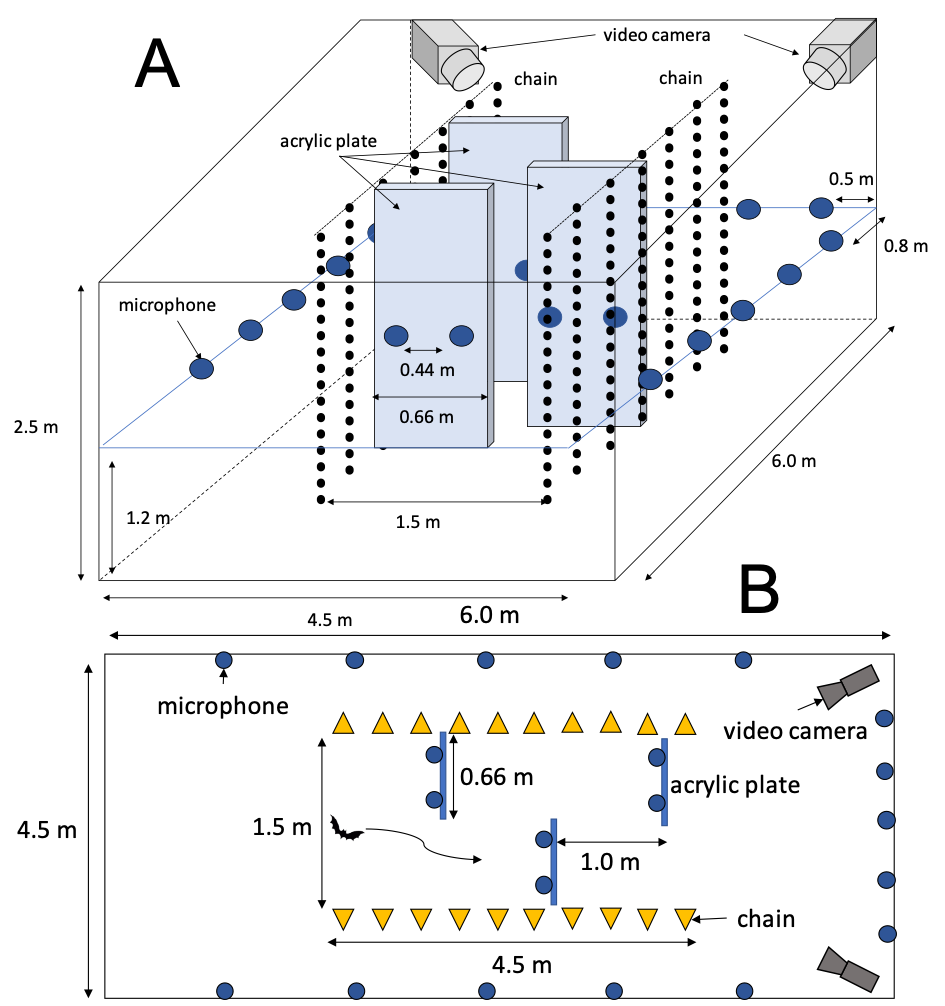
\includegraphics[width=15cm]{figures/top_view_measure.png}
  \caption{
    Top view of measurement system of flight trajectory,
    pulse direction.
  }
  \label{fig:top_view_measure}
\end{figure}
\vspace{\stretch{1}}

\newpage
\vspace*{\stretch{1}}
\begin{figure}[H]
  \centering
  \vfill
  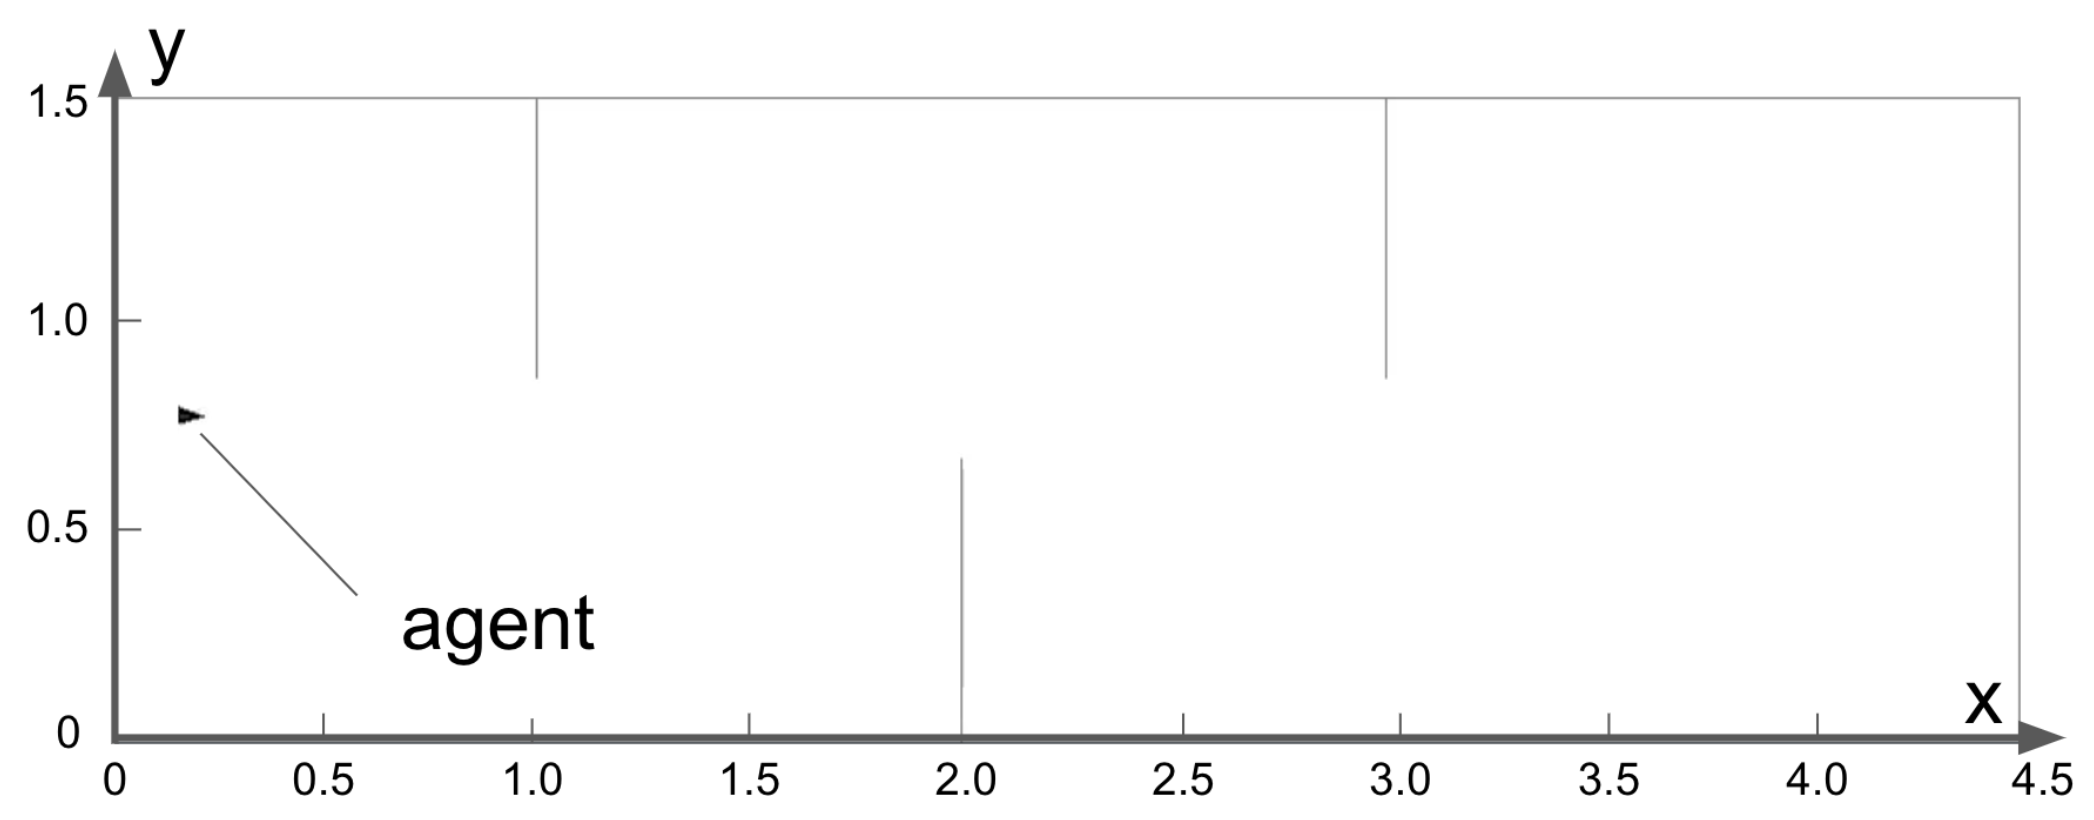
\includegraphics[width=15cm]{figures/simulation_field.png}
  \caption{
    Simulation field.
    Start point for agent is (0.2±0.05, 0.7±0.05).
    The gray lines are obstacles.
  }\label{fig:simulation_field}
\end{figure}
\vspace{\stretch{1}}

\newpage
\vspace*{\stretch{1}}
\begin{table}[H]
  \caption{A, Eの刺激周波数}\label{tab:ae}
  \centering
    \begin{tabular}{c|cl}
      Stimulus Number & Formant frequency\SI{}{[\hertz]} \\
          & F1 & F2 \\ \hline
      1 & 760 & 1080 \\
      2 & 731 & 1656\\
    \end{tabular}
\end{table}
\vspace{\stretch{1}}

\end{document}
